\documentclass[journal,10pt,letterpaper]{IEEEtran}
\usepackage[T1]{fontenc}
\usepackage{amsmath,amssymb,graphicx,booktabs,array,cite,url}
\usepackage[hidelinks]{hyperref}
\graphicspath{{figures/}}
\newcommand{\SE}{\mathrm{SE}(3)}
\newcommand{\NR}{\textit{NR}}
\newcommand{\placeholder}[1]{\textbf{[#1]}}
\hyphenation{local-ization regis-tration multi-start iner-tial}
\title{Gate-Aware Budgeted NDT Recovery for Prior-Map LiDAR--Inertial Localization}
\author{\placeholder{Author names and order to be approved}%
\thanks{\placeholder{Affiliations, postal addresses, and author e-mail addresses.}}%
\thanks{\placeholder{Corresponding author name and e-mail.}}%
\thanks{\placeholder{Funding agencies and grant numbers, or confirmation of no external funding.}}}
\markboth{MANUSCRIPT FOR ADVISOR REVIEW --- NOT SUBMITTED}{Gate-Aware Budgeted NDT Recovery}
\begin{document}
\maketitle
\begin{abstract}
Prior-map localization can lose useful measurements when a geometry check at an inaccurate prediction prevents registration from being attempted. We investigate the separation between pre-optimization screening and post-registration observation admission in a lidar--inertial system. The proposed pipeline preserves the native normal distributions transform optimizer and inertial filter, records pre-alignment geometry diagnostically, and admits measurements using unchanged post-registration quality criteria. Failed nominal matches can receive two fixed yaw restarts within a strict per-run computation budget. A controlled 60-scan causal ablation on Newer College uses real inertial propagation, scan deskewing, and delayed map-observation fusion. Removing the pre-optimization veto alone yields 60 converged registrations but no accepted map observation. Combining optimizer access with budgeted recovery reduces complete-window reference-relative translation and rotation root mean square errors from 7.986422 metres and 13.052649 degrees to 0.209943 metres and 2.984149 degrees, with eight additional registrations and 57 accepted observations. An earlier matched-segment map study records an 82.2 percent reduction in registration-process high-water memory, with timing and tail-error trade-offs. These results demonstrate a specific causal recovery mechanism on an exposed development window, rather than a new optimization principle or general accuracy guarantee. Evaluation uses a map-anchored reference with a conditional frame interpretation; robot deployment remains unverified.
\end{abstract}
\begin{IEEEkeywords}
Lidar--inertial localization, prior maps, normal distributions transform, observation admission, bounded recovery.
\end{IEEEkeywords}
\begin{center}
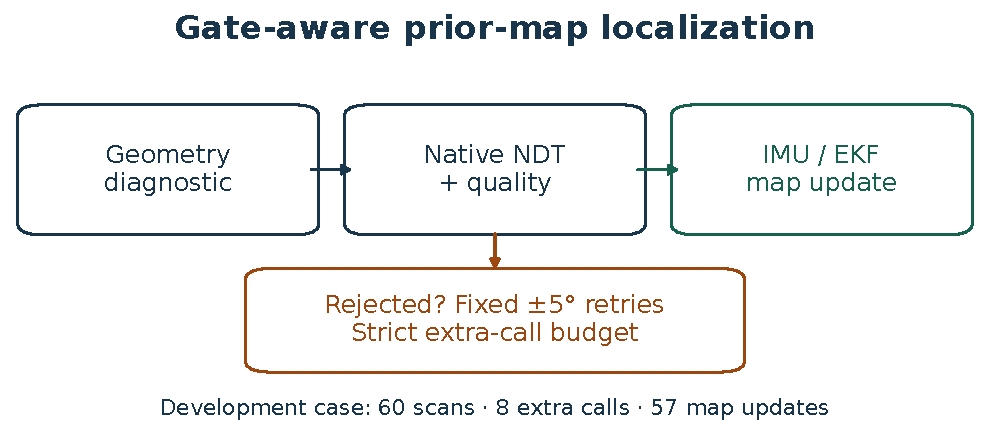
\includegraphics[width=\columnwidth]{gagraphic.pdf}
\par\smallskip\footnotesize\textit{Graphical abstract: diagnostic geometry, unchanged quality admission, and bounded retries form distinct stages of a causal inertial localization path.}
\end{center}

\section{Introduction}
\IEEEPARstart{L}{ocalization} against a fixed prior map can reduce the need for online map reconstruction, but reliable operation requires more than a successful registration call. The system must select valid map data, provide a causal initial pose, decide whether to attempt optimization, and determine whether its output is a suitable observation for the inertial estimator. Native normal distributions transform (NDT) remains useful for this architecture because it estimates a rigid alignment against Gaussian target geometry without requiring a newly designed solver~\cite{magnusson,pcl}.

A practical conflict arises when a pre-optimization geometry predicate is evaluated at an inaccurate prediction. Large nearest-map distances or low overlap may reflect initial misalignment rather than an absence of usable structure. A hard veto can then prevent both nominal registration and any recovery path from running. In contrast, allowing optimization does not imply that the result should be fused: a converged output can still fail post-registration quality checks. This distinction becomes consequential in a closed loop, where withholding a measurement changes the predictions used for subsequent scans.

We investigate this conflict in an existing NDT--inertial localization system. Geometry diagnostics remain unchanged, while their authority to prevent optimization is removed. The optimized result still faces the same basic and coverage-consistency criteria. Only a failed nominal result can trigger a fixed pair of yaw-restarted native alignments, and a run-level quota limits the additional work. Rejected observations are not replaced by artificial map measurements; the real inertial estimator continues propagating.

The contributions are limited to three experimentally supported points:
\begin{enumerate}
\item A gate-aware observation path separates map availability, pre-alignment diagnostics, optimized-pose admission, and bounded recovery around an unchanged native NDT solver and filter.
\item A controlled causal ablation with real inertial propagation shows that optimizer access alone is insufficient, whereas access plus eight extra alignments recovers a specific 60-scan perturbed-initialization case.
\item A resource-scoped evaluation reports local-target memory savings together with latency, maximum-error, reference, and deployment limitations, rather than claiming whole-system savings or universal recovery.
\end{enumerate}
The work does not introduce an NDT objective, a multistart optimization principle, or a new extended Kalman filter (EKF) model. Its contribution is an implementation-level responsibility change and a measured causal interaction.

\section{Related Work and Technical Positioning}
\subsection{Odometry and Fixed-Map Localization}
FAST-LIO2 uses direct point registration and an incremental spatial map within an iterated filtering architecture~\cite{fastlio2}. DLIO combines continuous-time motion correction, a geometric observer, and scan-to-submap registration~\cite{dlio}. STEAM-LIO and Singer-LIO investigate continuous-time inertial estimation with Gaussian-process motion priors~\cite{steam,singer}. Their Newer College odometry results supply useful context, but an incrementally built map and an aligned complete trajectory are different from externally anchored prior-map localization.

The closest systems already address important parts of this problem. 2Fast-2Lamaa supports mapping and localization in global or topometric maps with continuous distance fields~\cite{twofast}. SuperLoc assesses alignment risk and incorporates supporting pose priors before failure~\cite{superloc}. Koide \textit{et al.} jointly optimize scan-to-scan, scan-to-prior-map, and inertial factors in a sliding window~\cite{koide}. Autoware's NDT scan matcher documents prediction interpolation, registration-quality checks, initial-pose search, and optional multiple-initialization covariance estimation~\cite{autoware}. Reliability gating and multiple starts therefore cannot be claimed as inventions here.

\begin{table*}[t]
\caption{Closest Existing Methods and the Specific Difference Studied Here}
\label{tab:related}
\centering\footnotesize
\begin{tabular}{p{0.16\textwidth}p{0.36\textwidth}p{0.40\textwidth}}
\toprule
Existing system & Established mechanism & Difference and claim boundary of this study \\
\midrule
2Fast-2Lamaa~\cite{twofast} & Continuous-time undistortion; continuous distance-field scan-to-map localization; global/topometric targets. & Native Gaussian PCL NDT and the existing EKF are retained. We isolate the interaction of one pre-alignment veto with fixed-budget retries; no new map representation or accuracy superiority is claimed. \\
SuperLoc~\cite{superloc} & Predictive alignment risk, observability assessment, and active supporting-prior fusion. & We change the responsibility of a particular inherited distance/overlap veto. Our result neither invalidates predictive risk analysis nor demonstrates better degeneracy handling. \\
Koide \textit{et al.}~\cite{koide} & Joint scan-to-scan/map registration and IMU factors; sliding-window state estimation. & We preserve a separate NDT measurement and unchanged delayed EKF fusion, rather than introducing tighter coupling or a global initializer. \\
Autoware NDT~\cite{autoware} & Score/iteration/support diagnostics, pose validation, Monte Carlo initialization, and optional multi-start covariance estimation. & The tested intervention concerns optimizer reachability and event-only fixed yaw retries under one unchanged quality rule. It is not the first NDT reliability gate or multi-initialization implementation. \\
\bottomrule
\end{tabular}
\end{table*}

\subsection{Responsibility of Geometry and Quality}
Table~\ref{tab:related} distinguishes architecture from a numerical leaderboard. Our inherited pre-gate is not equivalent to SuperLoc's risk model or Autoware's complete diagnostics. We test whether that particular veto suppresses a useful optimization-and-admission sequence. Post-quality rejection remains active. Local map restriction, event triggering, and restarting are mature components; the manuscript's novelty is limited to a reproducible system-design finding and its controlled ablation. No head-to-head advantage over these systems has been measured.

\section{Gate-Aware Budgeted Measurement Path}
\subsection{Frames, Causality, and Inertial Continuity}
Let $T_{A,B}$ transform coordinates from frame $B$ to frame $A$. Registration returns the lidar pose in map frame $M$, while the filter state refers to IMU frame $I$. With fixed sensor transform $T_{I,L}$,
\begin{equation}
 T_{M,L}=T_{M,I}T_{I,L},\qquad
 T_{M,I}=T_{M,L}T_{I,L}^{-1}.
 \label{eq:frames}
\end{equation}
The same frozen extrinsic chain is used throughout. A window is initialized once from its anchor reference; a disturbed condition applies map-axis yaw $+8^\circ$ to the lidar attitude, preserves lidar position, and recomputes the IMU pose including the lever arm. Initial velocity and biases are inherited zero priors, not independently measured zero motion.

Subsequent initial poses $T_P$ come from actual causal IMU--EKF output. The node selects a delivered state at or before scan reference and uses the existing body-twist interface for at most 20~ms of projection. Current and future test-reference poses are unavailable to online decisions. Each method evolves its own history, so identical raw measurements need not produce identical deskewed coordinates after states diverge.

The scan header denotes scan start; the existing inertial deskew also references scan start. A delayed NDT observation retains that measurement time. The unchanged out-of-sequence measurement (OOSM) path updates the applicable historical state within its existing 20~ms alignment tolerance and replays real IMU samples to the current state. If no candidate is admitted, no map observation is published and inertial propagation continues. No second propagation model or new filter update is introduced.

\subsection{Native Registration and Local Targets}
The frozen source preprocessing uses 0.25~m voxels, 0.5--80~m range filtering, and a deterministic cap of 1,400 points. Native PCL NDT parameters are resolution 0.8~m, step size 0.08, transformation epsilon 0.001, at most 40 iterations, and outlier ratio 0.55. Every optimized candidate is a real native alignment; no post-processing pose inherits a fabricated convergence flag.

The existing local manager partitions a target prepared by two global 0.15~m voxel passes into 20~m horizontal tiles. It requests tiles intersecting source points projected by $T_P$, adds a 10~m safety margin, and uses a 30~m expanded selection at updates for hysteresis. Covered targets and Gaussian models are reused. Missing or corrupted required map assets remain hard failures. The visualization-map publisher is separate from the localization process and is excluded from reported two-node memory.

\subsection{Pre-Alignment Geometry as a Diagnostic}
For nearest-map distances $d$ at $T_P$, the original attempt predicate is
\begin{equation}
 \operatorname{median}(d)\leq 1.0\,\mathrm{m},\quad
 P_{90}(d)\leq3.0\,\mathrm{m},\quad O_{0.5}(T_P)\geq0.50.
 \label{eq:pregate}
\end{equation}
The old path returns before NDT if any term fails. The diagnostic-only geometry mode, denoted G, records the same statistics and predicate but permits registration when required inputs are valid. It does not lower a threshold, declare the prediction correct, or force an optimized result into the filter.

\subsection{Post-Registration Quality Admission}
The frozen coverage implementation partitions scanner azimuth into 16 sectors. Eight odd sectors form possible quality blocks; block activity is fixed by at least ten input points before candidate optimization. At least four active blocks and 300 even-sector points are required. For candidate $T$, define
\begin{align}
 L_b(T)&=\frac{1}{|S_b|}\sum_{p\in S_b}
 \min\!\left\{\frac{d(Tp,\mathcal M)^2}{(0.5\,\mathrm{m})^2},1\right\},
 \label{eq:block}\\
 Q(T)&=\frac{1}{|\mathcal A|}\sum_{b\in\mathcal A}L_b(T),
 \label{eq:quality}
\end{align}
where $\mathcal A$ is the active-block set and $\mathcal M$ the same target. Overlap is the fraction of active-block points within 0.5~m of the target. Missing blocks are unavailable evidence, not zero-loss samples.

A candidate must be finite, a valid rigid transform, natively converged, coverage-evaluable, and have overlap at least 0.50. The retained absolute quality rule additionally requires
\begin{equation}
 Q(T)\leq0.30.
 \label{eq:qgate}
\end{equation}
Because Full NDT uses these source points during registration, $Q$ is a \emph{Coverage Consistency Mean}, not an independent held-out validation loss. It is not a probability of correctness. Its threshold was developed on previously exposed data, not calibrated as a universal sensor-independent constant.

\subsection{Budgeted Native Retries}
The simple recovery component C first attempts one Full NDT alignment from $T_P$. If nominal quality fails and budget remains, it constructs two fixed initializations,
\begin{equation}
 R_\pm=R_z(\pm5^\circ)R_P,\qquad p_\pm=p_P.
 \label{eq:seeds}
\end{equation}
Only attitude changes; left-multiplying the full transform and rotating $p_P$ would implement a different operation. Each seed is optimized once against the same current source and target. The same basic and absolute quality conditions apply to every output.

C chooses the largest native transformation-probability score among admissible candidates. An exact tie is resolved by smaller prediction distance and then smaller fixed candidate ID, using
\begin{equation}
 r(T,T_P)=\sqrt{\left(\frac{\Delta t}{0.8\,\mathrm m}\right)^2+
 \left(\frac{\Delta\theta}{5^\circ}\right)^2}.
 \label{eq:tie}
\end{equation}
In the retained implementation, 0.8~m and $5^\circ$ are tie-break scales, \emph{not} hard candidate-to-prediction acceptance limits. A separate inherited publication limiter bounds adjacent NDT-observation steps by 0.5~m/$5^\circ$, and the existing EKF has its own update limits. Raw, selected, and published poses are distinct logged quantities.

At most two extra calls are permitted per event and twelve per approved 60-scan trajectory. This is a finite experimental quota, not an evaluated indefinite scheduler. If no output passes quality, the system publishes no map measurement. The G-only ablation follows the same path with the retry branch disabled. Figure~\ref{fig:path} shows the separation under test.

\begin{figure*}[t]
 \centering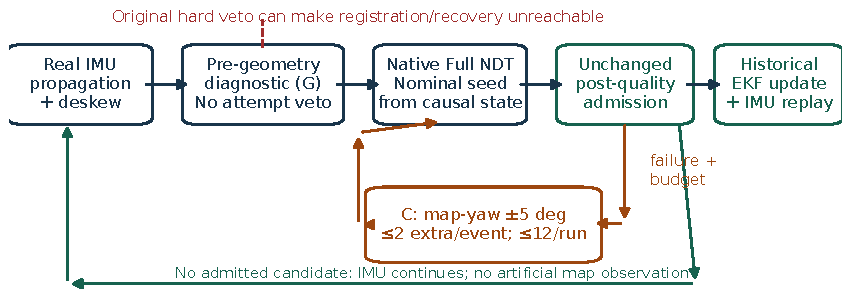
\includegraphics[width=\textwidth]{measurement_path.pdf}
 \caption{Causal observation path. G changes only the authority of the pre-alignment geometry predicate. All candidate outputs face unchanged post-registration quality, publication, and historical filter-update checks. A rejected scan leaves the real inertial estimator propagating. The dashed route illustrates the original early-return failure.}
 \label{fig:path}
\end{figure*}

\section{Experimental Protocol}
\subsection{Data, Reference, and Frame Limitation}
We use the original Newer College \texttt{01\_short\_experiment}, with Ouster OS1 lidar, its inertial measurements, and the supplied Leica prior~\cite{newer,ncindex}. The map is independently surveyed, but the official trajectory is generated by registering Ouster scans to that map~\cite{ncref}. We therefore report \emph{reference-relative pose error}, not independent motion-capture precision.

The historical Base interpretation is supported by the dataset paper and pinned robot-model evidence~\cite{newer,ncframe}, but its binding to the actual CSV is not certified. A dedicated follow-up verified that the local reference is the original 2020 Stereo-Cam release, with a retained official download identity and unchanged checksum. However, the official reference webpage assigns stereo poses to RS\_C1~\cite{ncref}, and the platform page defines RS\_C1 as optical while distinguishing a co-located robotics-axis Base~\cite{ncplatform}. The pinned robot description instead says that ground truth is expressed in Base~\cite{ncframe}. No inspected per-file metadata or exporter resolves this contradiction.

Let $T_{A B}$ map coordinates from $B$ into $A$, with $C$ the left optical frame, $B$ the robotics Base, $I$ the Ouster IMU and $L$ the cloud frame. The supplied Kalibr and Ouster calibrations give $T_{C I}$ and $T_{I L}$. The two documented interpretations imply different chains:
\begin{align}
 \text{Optical:}\quad T_{M L}&=T_{\mathrm{CSV}}T_{C I}T_{I L},\nonumber\\
 T_{M I}&=T_{\mathrm{CSV}}T_{C I},\label{eq:opticalchain}\\
 \text{Historical Base:}\quad T_{M L}&=T_{\mathrm{CSV}}T_{B C}T_{C I}T_{I L},\nonumber\\
 T_{M I}&=T_{\mathrm{CSV}}T_{B C}T_{C I}.\label{eq:basechain}
\end{align}
Co-location does not make $T_{B C}$ identity: its rotation changes optical axes into robotics axes. Both calibrated chains pass rigid-transform and inverse checks, which cannot certify CSV semantics. We do not switch interpretations by overlap, alignment fit, or minimum reference error. Historical errors below retain their explicitly conditional Base convention; they are not certified absolute accuracy. New reference-dependent experiments remain blocked until the exact-file convention is resolved.

\subsection{Controlled Causal Ablation}
The principal evaluation uses anchor raw2600 and the next 60 scans, raw2601--2660, with a $+8^\circ$ map-yaw initialization disturbance, denoted W1/C3. The compared runs use the same raw input, inertial model, calibration, deskew, initialization, native parameters, post-quality rule, and map-selection settings. Their actual target remains the same 2,297,615-point set. They differ only in enabling the geometry diagnostic mode and/or the fixed retries:
\begin{itemize}
 \item \textbf{Original}: the hard pre-geometry veto can prevent registration and recovery from being reached.
 \item \textbf{G-only}: optimization is reachable, but there are no extra initializations.
 \item \textbf{C+G}: optimization is reachable and the frozen budgeted retries are enabled.
\end{itemize}
All are actual independent causal executions. The original and C+G runs were previously sealed; the G-only ablation was executed separately, not synthesized from another run's states. W1/C0 and W3/C0 provide normal-initialization controls; W3 uses anchor raw6500. These are exposed development windows, not an independent confirmation of C+G or a global-relocalization benchmark.

An earlier matched 300-scan segment compares global and local target resource profiles. It has a different spatial footprint from the 60-scan recovery case and is not pooled with it. Historical optimizer-only experiments motivate the failure analysis, but their pose-history predictor is not substituted for the real inertial chain in the principal comparison. Supplementary Material separates those protocols and preserves negative evidence.

\subsection{Prospective Independent and External Comparisons}
Before any follow-up accuracy evaluation, the proposed anchor raw11000 was found to overlap the previously exposed raw10972--11032 interval. It was replaced deterministically by the next thousand-frame anchor after that interval, raw12000; the second anchor remains raw13500. Each proposed window contains one anchor and 60 evaluation scans. All 122 raw scan identities and integer timestamps were frozen without reading reference poses. Sparse earlier input-geometry screening is disclosed; these windows are not claimed to contain never-inspected geometry.

The planned comparison uses Original, G-only and C+G with normal and $+8^\circ$ initialization, each with an independent real IMU/filter history. This defines 12 prospective trajectories, not 12 completed runs. Source/target and anchor initialization remain unprepared behind the reference-frame gate. A finite feasibility inspection of FAST-LIO-LOCALIZATION~\cite{fastlioloc} found Python/Open3D interface mismatches without changing the installed environment. Available PCL GICP headers identify a possible controlled registration baseline, not a validated external localization system. Neither method has been run for a matched comparison.

\subsection{Evaluation and Resource Measurement}
Online outputs and decisions are frozen before reading test-reference values. With no per-method trajectory fit,
\begin{equation}
 e_t=\|p- p_{\rm ref}\|_2,\qquad
 e_R=\operatorname{angle}(R_{\rm ref}^{\mathsf T}R).
 \label{eq:errors}
\end{equation}
Each output is evaluated at its actual recorded state time. NDT uses scan reference; fused outputs can be approximately 100~ms later at the propagated IMU watermark. The frozen reference-matching rule permits bracketing gaps no larger than 150~ms or near endpoints within 50~ms. No offset is fitted. Rejected observations retain their actual propagated trajectory, rather than receiving zero error. A high-error output exceeds 0.5~m or $5^\circ$.

We report RMSE, 95th percentile and maximum, along with native calls, published observations and uninterrupted no-map spans. Node-callback time, initialization cost, and wall time have distinct scopes. Recent RSS is sampled every 50~ms for each node and their simultaneous sum; short peaks may be missed. The historical map study reports process high-water memory. The archived receipts do not establish a complete CPU model for every internal profile; it is not retrospectively inferred from the current workstation. Temporal dependence and single-run timing preclude broad statistical-significance or repeated-trial speed claims.

\section{Results}
\subsection{Optimizer Access Does Not Imply Admission}
Table~\ref{tab:ablation} reports the complete W1/C3 trajectory. The original path enters no NDT call because all 60 scans fail its pre-gate. G-only executes 60 native alignments, all converged, but no result passes unchanged post-quality admission. Its entire prediction and EKF pose sequences coincide with the original rejected-observation trajectory. Thus permitting optimization is insufficient in this case; native convergence and useful map updates are different outcomes.

\begin{table*}[t]
\caption{Controlled Causal Ablation: Complete 60-Scan W1/C3 Trajectory}
\label{tab:ablation}
\centering\footnotesize
\begin{tabular}{lrrrrrrr}
\toprule
Method & Position RMSE (m) & Rotation RMSE ($^\circ$) & Full nominal/extra & Map obs. & Rejected & High-error & Longest no-map \\
\midrule
Original & 7.986422 & 13.052649 & 0/0 & 0/60 & 60 & 60 & 60 \\
G-only & 7.986422 & 13.052649 & 60/0 & 0/60 & 60 & 60 & 60 \\
C+G & 0.209943 & 2.984149 & 60/8 & 57/60 & 3 & 2 & 2 \\
\bottomrule
\end{tabular}
\par\smallskip\raggedright
\textit{All comparisons use the same raw scans, target and model/quality settings, with separate real IMU/EKF histories. The original records zero attempts, not 60 failed alignments. G-only records 60 converged alignments but zero admissible map observations.}
\end{table*}

C+G first publishes a map observation at raw2603. Its fixed $-5^\circ$ restart produces $Q=0.296356$, satisfying the unchanged 0.30 gate. The subsequent filter history changes: raw2604 is rejected again, and raw2605 onward admits nominal measurements. The run publishes 57 observations and spends eight extra alignments. The first admitted map observation is also the first fused output that remains below the existing 0.5~m/$5^\circ$ reference-error criterion for the rest of the window. This recovery-time description is post hoc and never selects an online candidate.

The complete-window position RMSE falls from 7.986422 to 0.209943~m, and rotation RMSE from $13.052649^\circ$ to $2.984149^\circ$. The first two rotation errors remain large, approximately $11.245^\circ$ and $11.234^\circ$; the method does not remove the initial transient. Figure~\ref{fig:errors} includes every evaluated scan rather than only the favorable recovery interval. The result supports an additional contribution from retrying under this initial condition, rather than a benefit attributable to G alone.

\begin{figure*}[t]
 \centering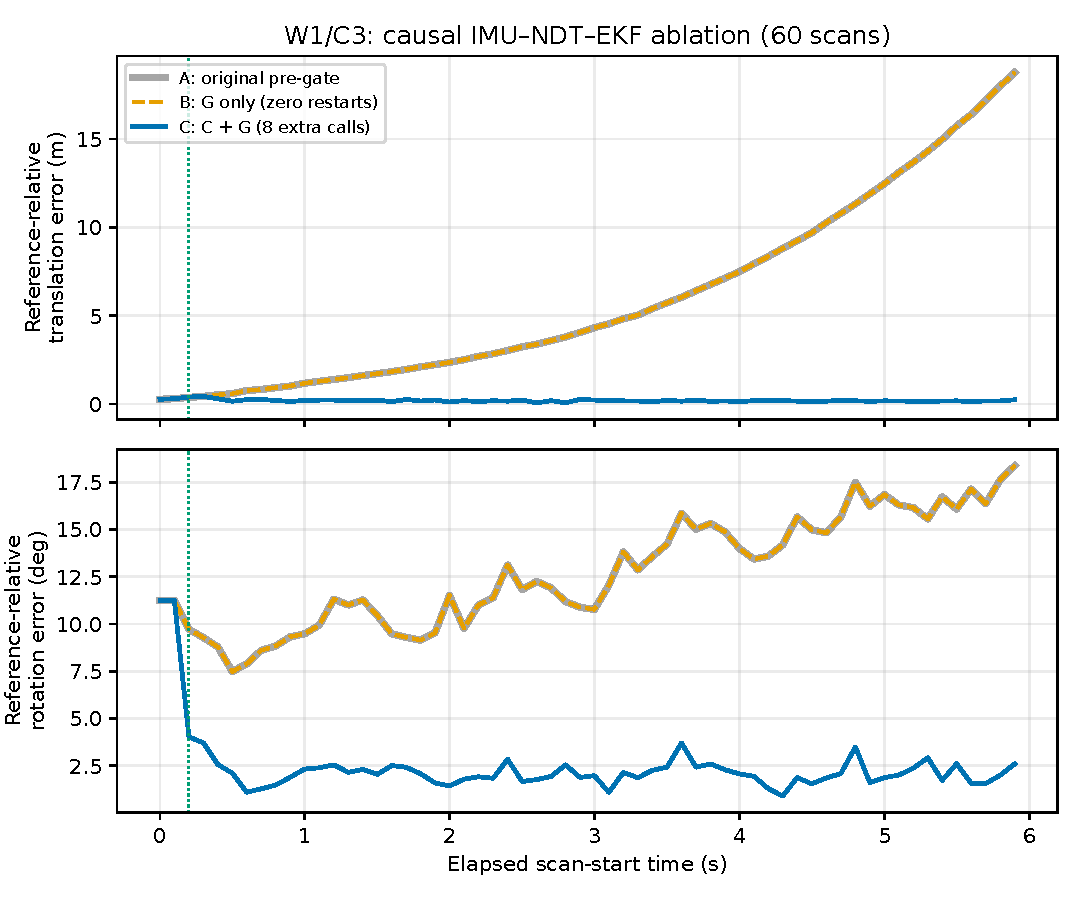
\includegraphics[width=0.92\textwidth]{ablation_errors.pdf}
 \caption{All 60 historical, conditional-Base reference-relative fused-state errors in W1/C3. Original and G-only trajectories coincide. The vertical marker identifies the first C+G map update at raw2603. The initial large rotation errors remain visible. The horizontal axis uses scan-start elapsed time; errors are evaluated at each output's actual fused-state time.}
 \label{fig:errors}
\end{figure*}

\subsection{Accuracy, Computation, and Normal Controls}
Table~\ref{tab:resources} preserves tail error and resource scopes. C+G uses 68 total alignments versus G-only's 60. Its observed callback mean is lower because the later causal optimization branch is different, not because multiple starts inherently reduce complexity. The first map/model construction contributes to maxima, and C+G's P95 exceeds 100~ms. No 10~Hz system certification follows.

\begin{table*}[t]
\caption{Accuracy Tails and Resource Cost in the Same W1/C3 Causal Comparison}
\label{tab:resources}
\centering\footnotesize
\begin{tabular}{lrrrrrr}
\toprule
Method & Position P95/max (m) & Rotation P95/max ($^\circ$) & Extra Full & Callback mean/P95/max (ms) & NDT peak (KiB) & Pair peak (KiB) \\
\midrule
Original &16.421686/18.755587&17.166246/18.375466&0&30.352/39.254/602.224&259060&282196\\
G-only &16.421686/18.755587&17.166246/18.375466&0&110.496/179.406/977.302&369136&389380\\
C+G &0.300124/0.444282&3.723287/11.245245&8&55.304/111.302/1006.031&369096&392536\\
\bottomrule
\end{tabular}
\par\smallskip\raggedright
\textit{Pair denotes simultaneously sampled NDT+EKF RSS, excluding publisher, deskew process, RViz and system memory. RMSE is given in Table~\ref{tab:ablation}. Single-run causal branches perform different work; no inter-method speedup is inferred.}
\end{table*}

Normal-initialization W1/C0 retains position/rotation RMSE 0.191979~m/$2.115287^\circ$ with and without G. W3/C0 likewise retains 0.175791~m/$2.009151^\circ$; its disturbed C3 result is 0.174696~m/$2.025760^\circ$. These unchanged control sequences establish no observed side effect in those runs, not safety outside the tested windows.

\subsection{Local-Map Memory Trade-Off}
In the separate matched 300-scan study, target restriction reduces active points from 3,142,751 to 552,716. Recorded NDT-process high-water memory decreases from 775,308 to 138,200~KiB, an observed 82.2\% reduction (Fig.~\ref{fig:memory}). This is a process-level result, not an 82.2\% whole-machine saving.

Position RMSE changes from 0.067985 to 0.061612~m, but position maximum rises from 0.119675 to 0.216396~m and rotation RMSE from $1.81802^\circ$ to $1.87495^\circ$. Steady alignment mean increases from 7.086 to 8.079~ms. Input-to-final-acknowledgment wall time is 33.82~s for a 29.90~s sensor span. Profiles are not an identical-binary kernel microbenchmark, and no live tile-boundary transition occurs. The larger recovery-window target explains why its roughly 360~MiB NDT RSS is not bounded by this earlier segment's lower footprint.

\begin{figure}[t]
 \centering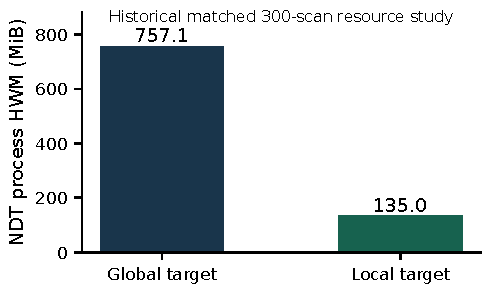
\includegraphics[width=\columnwidth]{local_map_memory.pdf}
 \caption{Historical matched-segment NDT-process high-water memory for global and restricted targets. The 82.2\% reduction does not include all localization/display processes and does not imply a universal target-independent budget. Timing and maximum-error trade-offs are reported in the text.}
 \label{fig:memory}
\end{figure}

\subsection{Published Reference Results, Not a Leaderboard}
Table~\ref{tab:published} reports published results for original Newer College Short, nominally 1530~s/about 1609~m. The names Short, 01-Short and 01\_short correspond to this original OS1 sequence~\cite{ncindex}. Two public author-output files each contain 15,301 timestamps exactly matching local PCD times. Nevertheless, equal sequence identity does not equate task, frame, initialization, sample set or alignment.

\begin{table*}[t]
\caption{Published Newer College Short Results Under Their Original Protocols}
\label{tab:published}
\centering\footnotesize
\begin{tabular}{p{0.24\textwidth}p{0.23\textwidth}rp{0.24\textwidth}l}
\toprule
Algorithm / result source & Task and position metric & Error (m) & Trajectory treatment & Original locator \\
\midrule
FAST-LIO2, run by Chen~\cite{dlio}&Odometry ATE RMSE&0.3775&evo; exact original alignment flags \NR&Table I\\
DLIO continuous~\cite{dlio}&Odometry ATE RMSE&0.3606&evo; exact original alignment flags \NR&Table I\\
STEAM-LIO~\cite{steam}&Odometry ATE RMSE&0.3042&Umeyama alignment&Table II\\
Singer-LIO~\cite{singer}&Odometry ATE RMSE&0.3020&Umeyama alignment&Table III\\
2Fast-2Lamaa~\cite{twofast}&Global-map odometry ATE RMSE&0.262&Umeyama alignment&Table 7\\
2Fast-2Lamaa~\cite{twofast}&Fixed-map localization position RMSE&0.128&Direct map-frame comparison&Table 7\\
\bottomrule
\end{tabular}
\par\smallskip\raggedright
\textit{These are full-sequence published contexts, not a matched ranking against our disturbed 60-scan map-localization case. \NR: not reported. Short-specific rotation RMSE is not provided in these tables.}
\end{table*}

The 2Fast comparison explicitly reuses FAST-LIO2 and DLIO results from Chen \textit{et al.}, and STEAM-LIO from Burnett \textit{et al.}; these are not independent reruns. Chen excludes the first 100 FAST-LIO2 poses on some sequences, without identifying the affected list in the inspected text. Its original alignment command is not specified, even though later compiled tables state Umeyama. No exact-protocol external ranking is therefore inferred.

The 0.128~m prior-map localization result is the closest task, but its complete duration, initialization, continuous map representation and pose convention differ from our disturbed window. Public STEAM/Singer trajectories establish time availability, not a certified Leica/body-frame transform or a matching disturbed initialization. No fitted transform is introduced to manufacture a fair-looking window score. The supplementary extraction retains original table/page locators and available versus unreported fields.

\subsection{Independent Causal Validation: Not Executed}
The reference-coordinate gate did not pass. Consequently, none of the 12 prospective independent causal trajectories was executed, and no new recovery rate, normal-initialization safety result or reference-relative error is reported. Non-execution must not be interpreted as a non-triggering successful run. The development-case results in Tables~\ref{tab:ablation} and~\ref{tab:resources} are preserved and are not upgraded into independent confirmation.

\subsection{Matched External Baseline: Not Established}
Only upstream-source and installed-environment feasibility were checked. No external algorithm was compiled or run, and no matched-baseline accuracy table is available. Published full-sequence numbers in Table~\ref{tab:published} remain contextual results under different protocols. They cannot support a state-of-the-art ranking for the proposed disturbed-window experiment.

\section{Discussion and Limitations}
\subsection{What the Causal Ablation Establishes}
The inherited pre-veto makes a registration/recovery path unreachable. G-only then separates that reachability issue from optimized-observation admission: all nominal optimizations converge but none can update the filter. C+G supplies an admissible alternative initialization, changes the actual history and reduces complete-window reference-relative error. This is stronger than reordering previously frozen per-frame outputs, but remains one known development failure with limited normal controls. It does not prove strict local minima or universal initialization-basin recovery.

Published systems already implement robust fusion, scan-quality assessment and multiple initializations. The actual finding is an interaction between two responsibility boundaries in this implementation, not the invention of those components. A directly comparable external prior-map experiment is absent; Table~\ref{tab:published} supplies context and cannot establish state-of-the-art accuracy.

\subsection{Negative Evidence and Deployment Boundary}
A fixed absolute quality gate can reject a reference-improving candidate. Conversely, an explored relative-only admission rule produced a normal-initialization counterexample: position RMSE rose from 0.211401 to 0.242043~m and high-error outputs from two to five. That rule is excluded, rather than repaired by fitting an additional threshold. A tested correction-history synchronization extension did not produce a subsequently consumed corrected prediction sample; no improvement is attributed to it. Supplementary Material preserves these findings without presenting rejected mechanisms as contributions.

The decisive window was already exposed during development, the accepted restart is near the quality threshold, and no retuned threshold or robustness sweep is used to enhance the result. The finite quota does not demonstrate indefinite operation. The map-anchored reference and unresolved exact-file pose convention limit accuracy conclusions. Resolving the conflict requires authoritative exporter metadata or a file-specific clarification, rather than choosing the transform that produces smaller errors. If that evidence identifies an error in the historical interpretation, every affected reference evaluation must be recomputed as a new version while retaining the original logs. A changed initialization convention also affects the causal experiment itself; re-evaluating old outputs alone cannot recreate a corrected run. There are no repeated independent trials or cross-dataset generalization evidence for C+G.

A real quadruped dataset and FAST-LIVO2 prior are available, but the physical lidar--IMU transform provenance is not established. The historical identity/zero fallback is not a calibrated extrinsic. No new robot baseline/C+G experiment or independent physical accuracy result is claimed; the unqualified transfer of the 0.30 consistency threshold to that sensor is also unverified. This unresolved deployment test does not alter the public-data ablation, but it prevents a deployment-ready claim.

\section{Conclusion}
We studied a gate-aware, budgeted observation path for prior-map lidar--inertial localization while retaining the native NDT optimizer and existing filter. In a complete 60-scan causal development case, diagnostic-only pre-geometry screening alone yields no admissible map update despite 60 converged registrations. The same access change combined with fixed yaw retries admits 57 observations using eight extra alignments and reduces position/rotation RMSE to 0.209943~m/$2.984149^\circ$. A separate matched-segment study records 82.2\% lower NDT-process high-water memory with explicit latency and tail-error trade-offs. The supported contribution is a reproducible responsibility-boundary and recovery interaction, subject to reference/frame uncertainty, limited validation scope and incomplete robot deployment. The follow-up coordinate-verification gate remains blocked, so neither independent recovery confirmation nor a matched external comparison has been established. The current manuscript is for advisor review with these prerequisites explicit, rather than an accuracy claim ready for formal submission. No external state-of-the-art superiority or new optimization theory is established.

\section*{Data and Software Availability}
Newer College scans, calibration and surveyed prior are distributed by the dataset authors~\cite{newer,ncindex,ncref} under their terms. Exact window identities, decision logs and source fingerprints are retained in the research archive. \placeholder{Authors must confirm the public archival repository/DOI, release permissions, and immutable software revision before submission.} This draft does not claim that the present submission package or all experimental outputs have already been uploaded. The local reproducibility supplement identifies historical code and evidence without redistributing the large dataset.

\section*{Acknowledgment}
OpenAI Codex/ChatGPT assisted in drafting and restructuring the manuscript text, preparing literature-extraction summaries, and generating plotting/typesetting code for the manuscript and graphical abstract. The experimental values were drawn from the frozen research archives rather than generated by the writing assistant. \placeholder{Authors must verify the exact AI tool/version and scope, complete any additional disclosure, and approve all scientific content and funding acknowledgments.}

\bibliographystyle{IEEEtran}
\bibliography{REFERENCES}
\end{document}
